\documentclass{article}
\usepackage{amsmath}
\usepackage[utf8]{inputenc}
\usepackage{graphics}
\usepackage{hyperref}
\usepackage[titletoc]{appendix}
\numberwithin{equation}{section}

% Sets path for all images includes
\graphicspath{ {images/}}
\usepackage{graphicx} %package to manage images

\usepackage[rightcaption]{sidecap}

\usepackage{listings} 
\usepackage{xcolor}
\usepackage{wrapfig}

\definecolor{codegreen}{rgb}{0,0.6,0}
\definecolor{codegray}{rgb}{0.5,0.5,0.5}
\definecolor{codepurple}{rgb}{0.58,0,0.82}
\definecolor{backcolour}{rgb}{0.95,0.95,0.92}

\lstdefinestyle{mystyle}{
    backgroundcolor=\color{backcolour},   
    commentstyle=\color{codegreen},
    keywordstyle=\color{magenta},
    numberstyle=\tiny\color{codegray},
    stringstyle=\color{codepurple},
    basicstyle=\ttfamily\footnotesize,
    breakatwhitespace=false,         
    breaklines=true,                 
    captionpos=b,                    
    keepspaces=true,                 
    numbers=left,                    
    numbersep=5pt,                  
    showspaces=false,                
    showstringspaces=false,
    showtabs=false,                  
    tabsize=2
}

\lstset{style=mystyle}
\lstset{language=R}

%\usepackage{showframe} % This line can be used to clearly show the new margins
\usepackage[margin=1.3in]{geometry}
\newcommand{\eqname}[1]{\tag*{#1}}% Tag equation with name

\begin{document}

\title{	
	\normalfont\normalsize
	\textsc{University of California, Davis} \\ % Your university, school and/or department name(s)
	\vspace{25pt} % Whitespace
	\rule{\linewidth}{0.5pt} \\ % Thin top horizontal rule
	\vspace{20pt} % Whitespace
	{\huge ECS 132 Term Project} \\ % The assignment title
	\vspace{12pt} % Whitespace
	\rule{\linewidth}{2pt} \\ % Thick bottom horizontal rule
	\vspace{12pt} % Whitespace
}

\author{Rohan Skariah \and Nathan Krieger \and Raymond Laughrey \and Geoffrey Cook}
\date{\normalsize\today}
\maketitle


\newpage

\section{Part A: Scavenger Hunt}

\subsection{Team Member 1: Nathan Krieger}

For my investigation of p-values being used in an academic setting I evaluated a paper titled "Does Professor Quality Matter? Evidence from Random Assignment of Students to Professors". The UC Davis professor that is a author is Scott Carrel from the department of Economics. The link to the paper will be provided at the end. 

The study aims to find if there is a relationship between a postsecondary level teacher's characteristics and student success at elementary and secondary levels. In order to analyze data that does not have measurement issues due to "self-selection" data was collected from United States Air Force Academy (USAFA) which randomly assigns students to professors and additionally has little to no difference in class material from different professors teaching the same course. 

In this study, the use of p-values arises when the assignment of student to professors is tested with significance tests. The basic idea was to reject the null hypothesis if it was found that there was nonrandom assignment of professors into course sections. A specific quote from the study that highlighted a possible over reliance on p-values was "Of the 36 estimated coefficients, none are statistically significant at the 5 percent level.". It seemed in this case while a p-value could be helpful in determining randomness, a confidence interval in addition or in place of the p-value/ hypothesis test could have provided a better insight as how random the assignment of the professors to a course was instead of just if the hypothesis seemed to be correct. Specifically, a confidence interval would of provided an actual interval of values that represent the randomness through the different cohorts. Additionally, the phrase "none are statistically significant" can be misleading as the word significant does not imply importance. Lastly, the ASA notes in their report on p-values says "values do not measure the probability that the studied hypothesis is true, or the probability that the data were produced by random chance alone" so it  is possible here that the randomness of assignment, which is integral to the data not having self-selection issues, could in fact have some non-randomness which could be missed by testing the null hypothesis alone. 

Link to Paper(Must be connected to UC Davis Library VPN): \href{https://www.journals.uchicago.edu/doi/pdfplus/10.1086\%2F653808}{Does Professor Quality Matter? Evidence from
Random Assignment of Students to Professors}

\subsection{Team Member 2: Rohan Skariah}

In a study published in 2001 titled "Canine atopic dermatitis: a retrospective study of 266 cases examined at the University of California, Davis, 1992–1998. Part I. Clinical features and allergy testing results" , Philip H. Kass, in combination with 3 other individuals, tried to analyze the significance of outside forces and atopic dermatitis on the type of allergies and infections they have. Philip H. Kass is a professor of Population Health and Reproduction at UC Davis. In this study, a sample of 266 dogs were used to perform these analyses. The crutial thing to understand to start the study is that "Canine atopic dermatitis is the clinical disease seen in atopic dogs that results from the release of inflammatory mediators, thereby causing clinically relevant allergic reactions to environmental antigens." Using this data, they can theoretically predict whether a certain bread of dog is at a greater risk of mould vs weeds etc. The data for this study was collected from 1992–98 at Veterinary Medicine Teaching Hospital of the University of California at Davis. 
In the analysis of the study, it is noted that "Values of  P less than 0.05 were considered statistically significant," which implies they relied heavily on p-values to consider data useful or not. The analysis talked about many aspects of the dog, and I will reference where they talked about p-values in each and why confidence intervals would have been better. \\

\boldsymbol{Breeds} When comparing the breed of dog that was most likely to have atopic dermatitis, statements like a the proportion of certain breed of dog having the disease was "higher than expected ( P less than 0.05)" appeared quite often. They were comparing the study results to the hospital population, but that provides little factual information to the study itself. However, using confidence intervals, you would be able to see the outliers in the study and consequently disregard them or treat them accordingly. \boldsymbol{Clinical \ signs} This section relied heavily on p-values to show the importance of certain values from the data. Statements like "There was a highly significant reverse correlation (P = 0.0025)" and "There was a very highly significant positive correlation between the clinical diagnosis of FAD and positive reactions to flea extract in allergy testing (P less than 0.0001)" gave the bases for the studies conclusions. 
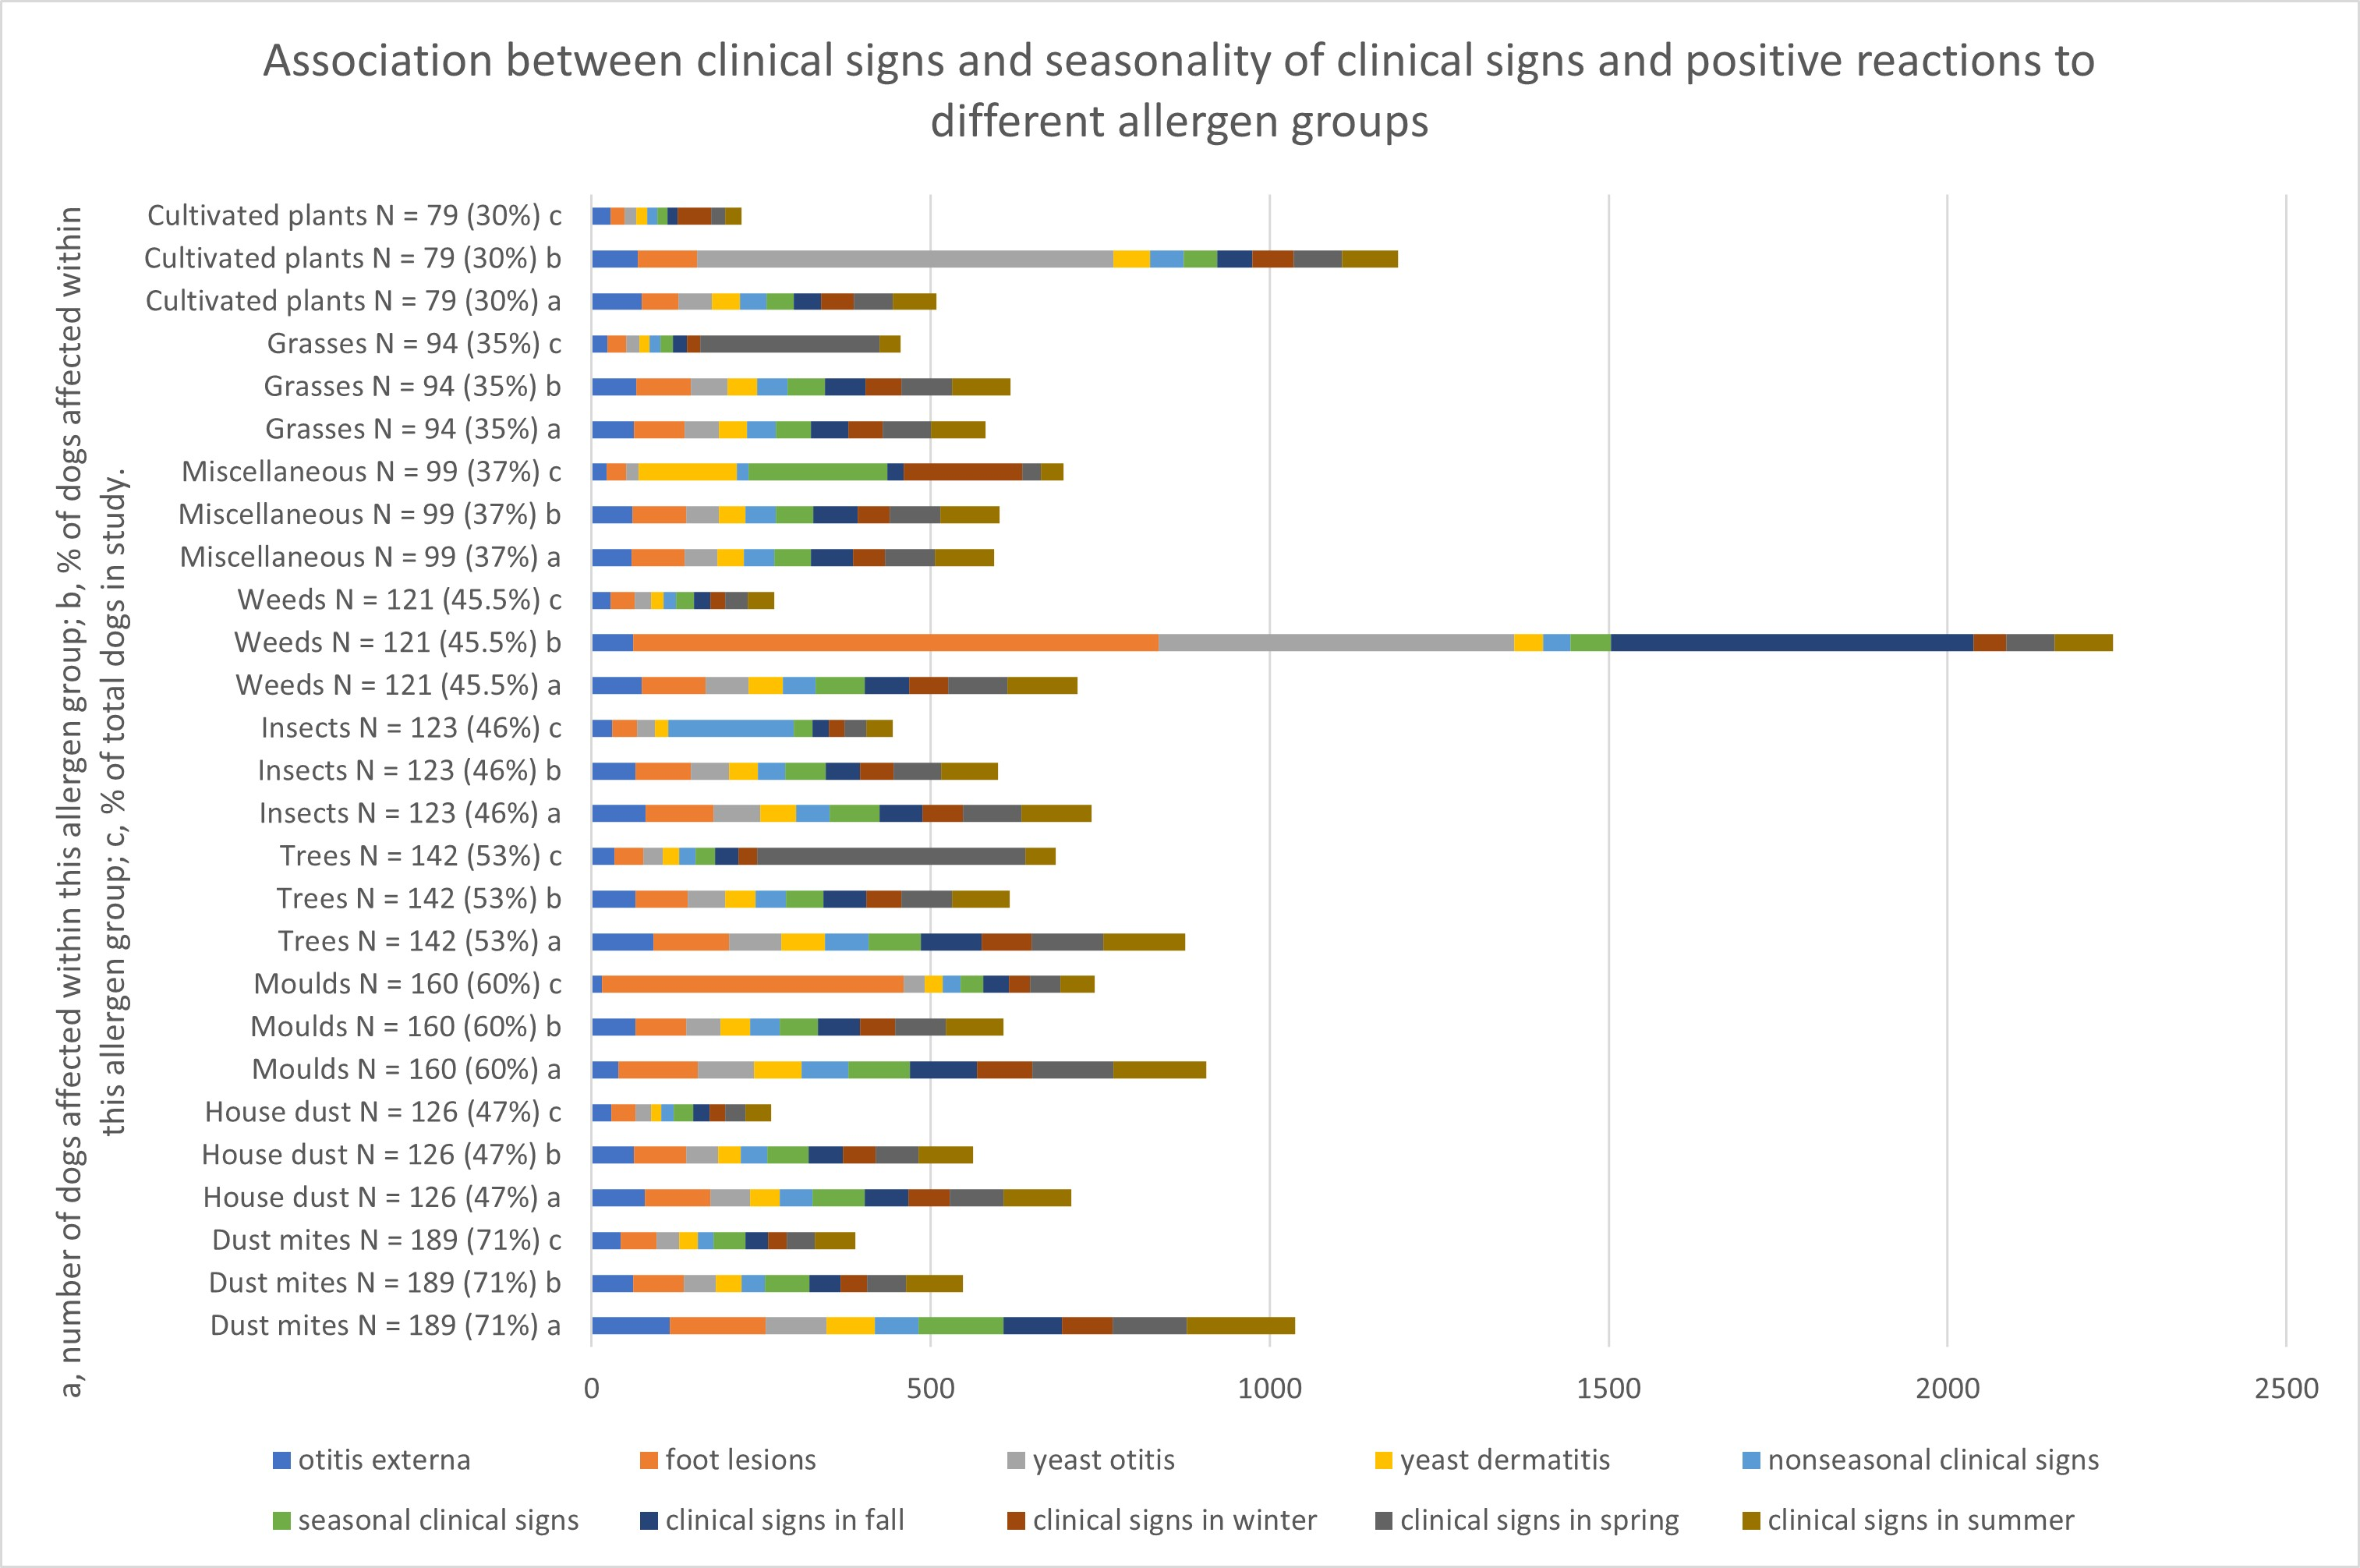
\includegraphics[scale = 0.6]{Association between clinical signs and seasonality of clinical signs and positive reactions to different allergen groups.jpg}

Many of these statements mislead the readers into valuing certain data points or conclusions over others. Even in the case above, almost every data column had some assertion about the significance of the values "*P less than 0.05; †P less than 0.01; ‡P less than 0.1". The graph shows little indication of significance except in the context of confidence intervals (where some of the values seem to be outliers). As a matter of fact, noting those values and making conclusions on why they differ from the rest seems like a better method of analysis that before. Please refer to the \href{https://onlinelibrary.wiley.com/doi/full/10.1046/j.1365-3164.2002.00285.x#t3}{TABLE} for the pure data and the associated p-values for each. It should be noted that the authors do \textit{try} to use confidence intervals for their data, but they over relied on p-values instead of confidence intervals. Correlating P less than 0.0001 and "highly significant positive correlation" is incorrect and won't benefit anyone. Moreover, since they are only using 266 dogs, and many calculations takes a subset of that sample, there isn't enough data to make a factual, educated, and reliable inference about the entire population on specifics like mould reacting to a breed of dog with atopic dermatitis. Using confidence intervals can give better information on how far off each breed of dogs or their characteristics are from the mean and how accurate they are, which is more informative than p-value testing.

Here is the link to the article: \url{https://onlinelibrary.wiley.com/doi/epdf/10.1046/j.1365-3164.2002.00285.x}

\subsection{Team Member 3: Geoffrey Cook}
For my examination of significance testing I found a paper with several authors including Dr. Peter J. Havel, a "Professor with joint appointments in the Departments of Molecular Biosciences and Nutrition" at UC Davis.  In a study published in 2008, titled "Development and characterization of a novel rat model of type 2 diabetes mellitus: the UC Davis type 2 diabetes mellitus UCD-T2DM rat," Dr. Havel attempted to create a model for rats with type 2 diabetes that "more closely models the pathophysiology of T2DM in humans."

This was accomplished by breeding rats in which both parents either already had type 2 diabetes or later developed it.  That way all rats bred after what they call the "F7 generation" had a "genetic propensity to develop diabetes." In an 18 month study biological markers, such as weight and hormone levels, were monitored in 16 males rats from generation F9 and F10 both before and after they developed diabetes. 

The use of p-values comes from the statistics and data analysis section.  They use p-values to compare several different values including body weight, energy intake, and age of onset of diabetes. The authors state that "differences were considered significant at P < 0.05." This is a misuse of the word significant and provides little information to the reader. However had they given the confidence interval, depending upon the range of the confidence interval, the significance is more explicit. A great example of this is actually provided in the paper when the authors state that "The incidence of diabetes in male and female rats in the F7 generation was 91.9 percent (102/111) and 42.6 percent (40/94) respectively, with the average age of onset being 183 ± 10 days in males and 286 ± 17 days in females     (P <0.0001, males vs. females)." Knowing that average age of onset is 183 ± 10 days in male rats is much more useful information than the fact that     P < 0.0001 which makes it "very highly significant."  The authors should provide more confidence intervals and not rely on p values as frequently, as confidence intervals provide much more insight about the data gathered. According to Ron Wasserstein, the ASA’s executive director, “Well-reasoned statistical arguments contain much more than the value of a single number and whether that number exceeds an arbitrary threshold. The ASA statement is intended to steer research into a ‘post p<0.05 era.’”

Here is the link to the article: \url{https://journals.physiology.org/doi/full/10.1152/ajpregu.90635.2008}
\subsection{Team Member 4: Raymond Laughrey}

My paper including p-values is about testing a drug Memantine (a current FDA approved treatment for Alzheimer’s) on its efficacy to treat Ataxia syndrome, tremors in people usually above age 50. The research is a double-blind placebo-controlled test over one year. The outcome of the trials was measured with the Behavioral Dyscontrol Scale (BDS) and CATSYS intention tremor severity. This research was conducted by multiple Phd. and MDs from UCDavis’ department of medicine.

Over the course of one year, thirty-four patients were given Memantine, thirty-six were given placebos. After the year, no effects were found for the BDS score, with the memantine group mean SD score at 16.12 from 17.44 compared to the placebo group mean 15.72, from 15.66 (p=.727). This is tested specifically for larger motor control functions, like grasping objects and pressing large buttons. They emphasize that there are no significant improvements over the course of the treatment, citing P-Values instead of a confidence interval. The CATSYS writing severity, and hand/finger tapping outcomes look slightly better. Memantine improved to a .37 score from .51, while placebos mean was precisely .72 both before and after a year, (p =.087).

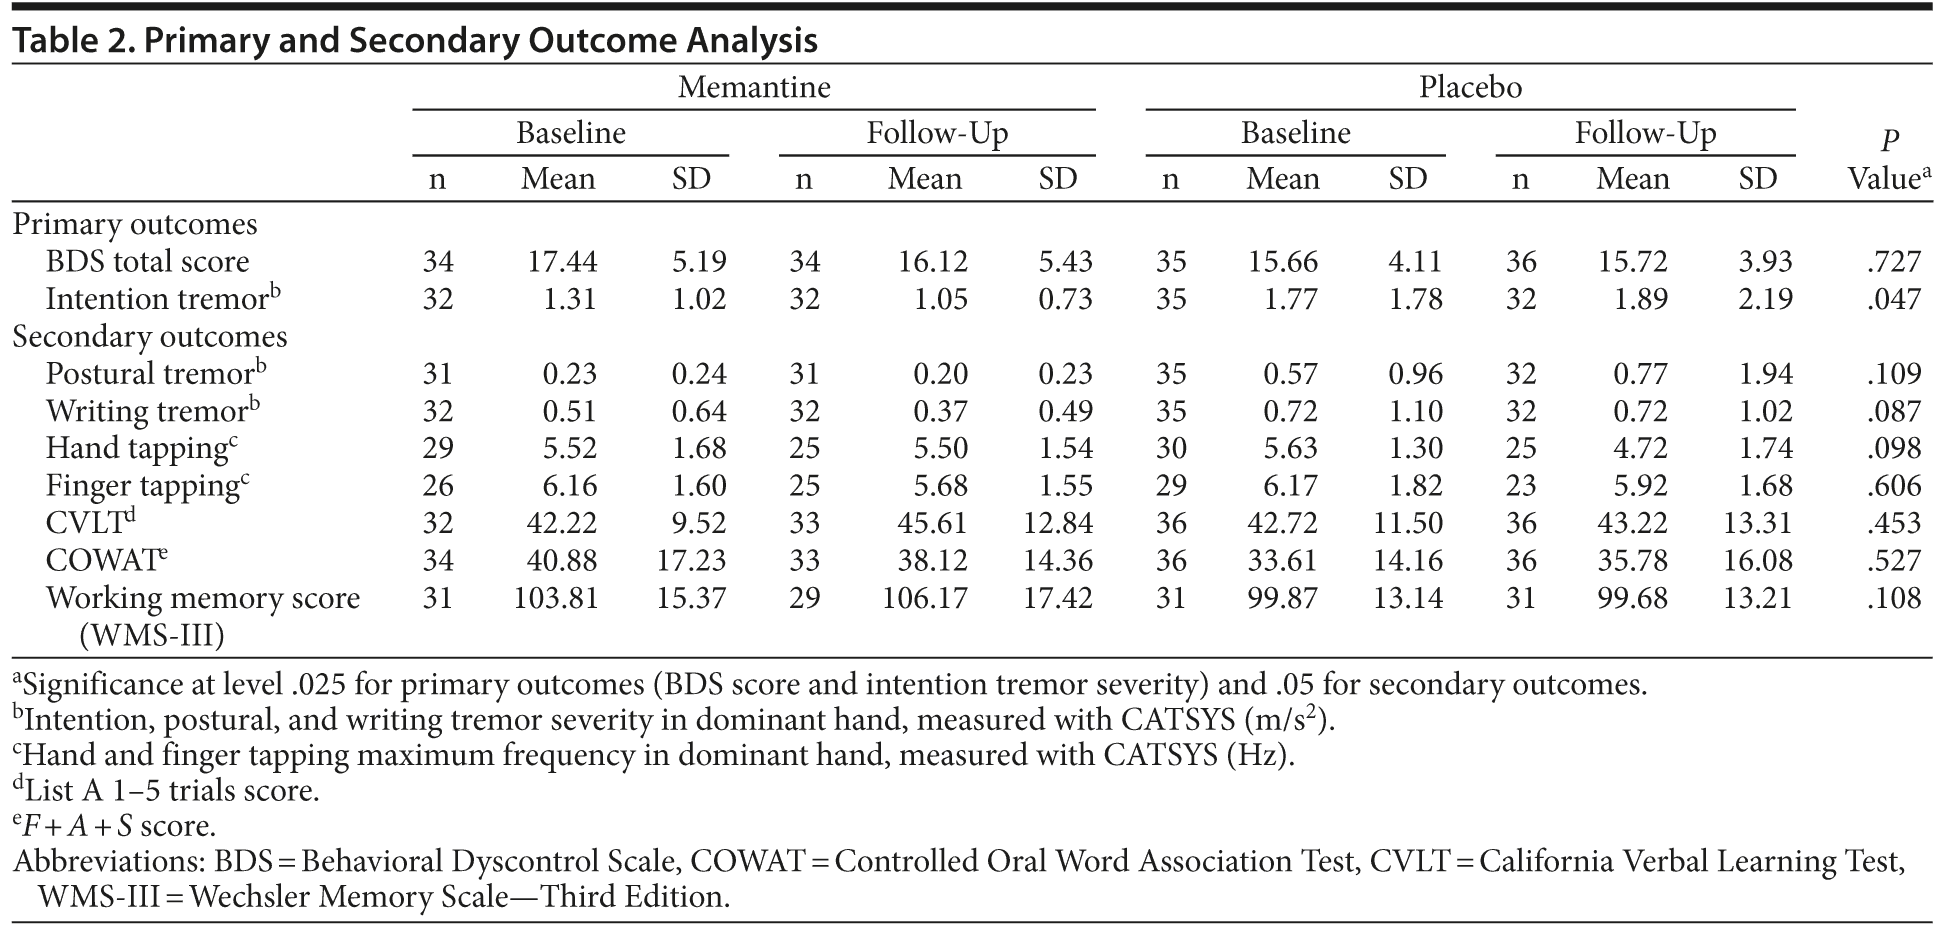
\includegraphics[scale=0.3]{RayTable.png}

These results can appear somewhat promising for improvement in fine motor control but the use of p-values as a measure of the larger motor control functions being a high value makes the improvements seem trivial. Even if the medication can only help slightly, something is better than nothing, especially considering the progressive and adverse nature of tremors as age progresses. Calculating the confidence interval for the BDS tests with a sample size of thirty-four, standard deviation of 5.43, is between 13.9 and 17.6. The difference between score improvements in the whole numbers can mean a world of difference in a real-world scenario, for example, a healthy college aged student scores at 17.6 compared to healthy elderly at 14.7.
Link: https://www.psychiatrist.com/jcp/neurologic/neurology/memantine-fragile-xassociated-tremorataxia-syndrome/

\newpage

\section{Part B: Porto Taxi Trip Data}

\subsection{Data Importing}

\begin{lstlisting}
    train <- read.csv('train.csv')
    numRowsToCalculate <- 10000 
    # Indicate the sample size and sample the train data
    chunk1 <- train[sample(nrow(train), numRowsToCalculate), ]
\end{lstlisting}

\subsection{Libraries Used}

library(regtools)    --qe wrapper functions for ML and prediction\\
library(datetime)    --converting from UNIX timestamp\\
library(rjson)    --Reading polyline data into GPS coordinates\\
library(data.table)  --Turning data into table\\
library(randomForest)    --Used for qeRF()\\
library(gbm)    --Used for qeGBoost()\\
library(keras)    --Used for qeNeural()\\
library(glmnet)    --Used for qeLasso()\\
library(tensorflow)    --Used for qeNeural()\\
library(ggplot2)    --Used for plotting mean call type duration.\\
library(rcompanion)    --Used for lm()\\

\subsection{Unused/Messy Data}
Trips lasting less than 15 seconds were discarded as errors in reporting or outliers to prevent data from being skewed too far in the low direction. This makes logical sense as it is highly unlikely anyone would take a taxi trip for 15 seconds.

\subsection{Data Analysis}
We used a random sample of 10,000 trips from each call type to calculate trip duration density, and mean of each type. When calculating the estimated busy time density, we specified a number of rows to calculate a consistent busy time week over week. Trip times that overlapped were also discarded to not double-up on busy time, assuming the taxi had multiple occupants with different destinations.

\subsection{Let T denote trip duration. Explore finding a model for $f_{T}$ from one of our density families.}

%Summing the duration of all trips from all trip types, We found that gamma distribution model fit the trip duration, using 'alpha <- (mean(x)^2)/var(x), beta <- (mean(x))/var(x) code here' we were able to find the alpha and betas of the function.
%


After inspection of the provided data set our group decided to leverage the GPS data in order to derive trip duration's. First we split the GPS data into individual trips and then, using the fact each GPS entry is 15 seconds, we found the overall trip time by multiplying by the number of entries by 15. In order to visualize the data we graphed the histogram of the data using a random sample of 10,000 rows.

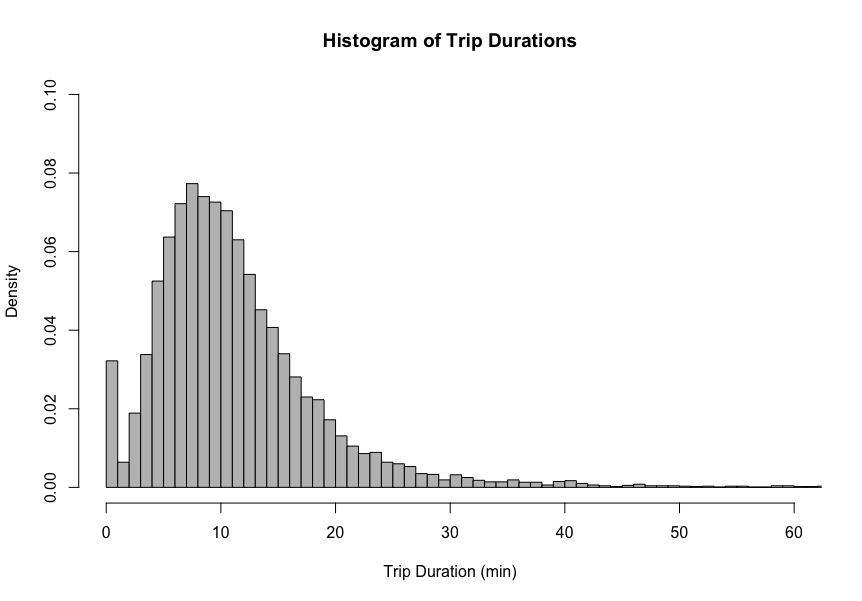
\includegraphics[scale=0.5]{raw_data_histogram_trip.png}

From the histogram it's clear there is a large number of values near zero. After further inspection of the data it is clear there are several values that are too small to be true. Such as values of 0 for trip time. So in order to not distort calculation which would effect our parameter fitting we excluded all trip times less than fifteen seconds and graphed the histogram

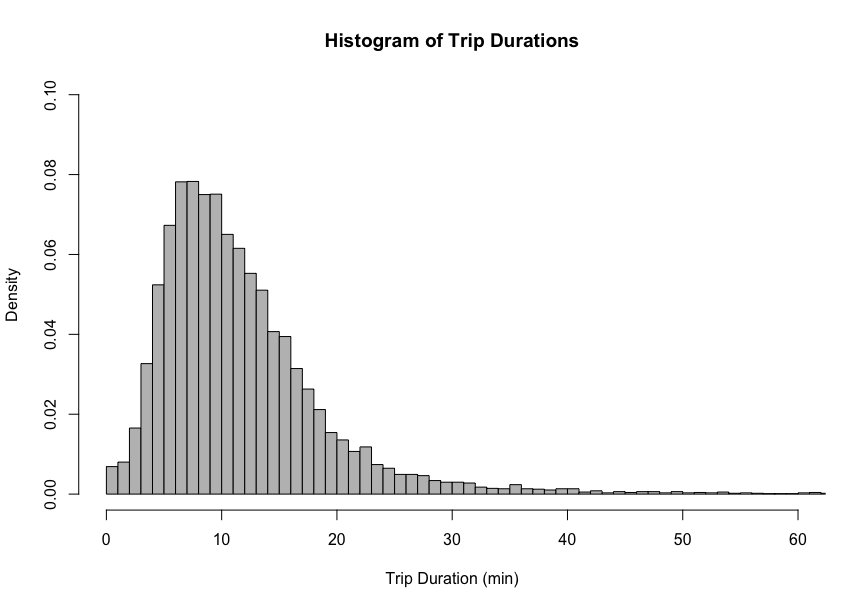
\includegraphics[scale=0.5]{clean_data_no_curve.png}

Noting the data has similar characteristics to a gamma distribution: a steep incline near zero and a tapering off for larger values. We decided to fit a gamma distribution to the data using both method of moments and iterative estimation of the parameters. In addition, we tried to fit a normal distribution to the data with the following results. 

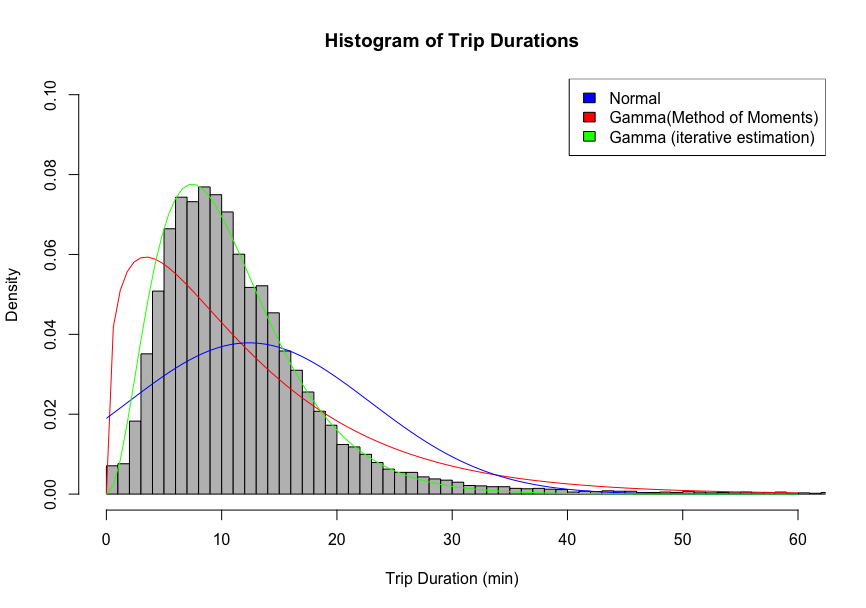
\includegraphics[scale=0.5]{normal_vs_gamma(mm)_gamma(iterative).png}

From the three curves it seems the iterative estimation gets the closest to fitting the data. However, there is a possibility of over-fitting to sample we used. Because of this we tested the iterative estimation density with several samples and found the parameters fit many different samples. The density's for the curves are noted below:

\begin{equation}
    Normal \rightarrow  f_T(t) = \frac{1}{\sqrt{2\pi} \sigma}e^{-0.5(\frac{t-\mu}{\sigma}^2)}
\end{equation}
\begin{equation}
    Gamma (\text{Method Of Moments}) \rightarrow f_T(t) = \frac{1}{\Gamma(r)} \lambda^r t^{r-1}e^{-\lambda t}, t > 0
\end{equation}

\begin{equation}
    Gamma (\text{Iterative Estimation}) \rightarrow f_T(t) = \frac{1}{\Gamma(r)} \lambda^r t^{r-1}e^{-\lambda t}, t > 0
\end{equation}

where the rate and shape parameters are found by using the method of moments equations for the Gamma Distribution: 

\begin{equation}
    \lambda_{est} = \frac{M_1}{s^2}
\end{equation}

\begin{equation}
    r_{est} = \frac{M_1^2}{s^2}
\end{equation}

Additionally, the rate and shape for the iterative estimation method are as follows: 

\begin{equation}
    \lambda_{est} = \frac{3.75}{\bar{X}}
\end{equation}
\begin{equation}
     r_{est} = 3.25
\end{equation}

Noting that $\bar{X}$ is defined as the sample mean for the given sample population.

\newpage

% \appendix \section{yes}`1
\newpage

\subsection{Let B denote the proportion of time a driver is busy, i.e. actually driving rather than waiting for the next fare. Explore finding a model for $f_B$ from one of our density families.}

We could not use a random sample from the data set for this part as the dates of trips varied greatly and did not provide enough trip data to determine how busy a driver was given a time interval.  For finding a model of the proportion of time a driver is busy we used the first 10,000 rows of the data set and split them by taxi number.  We then calculated that taxi id's busy time by summing the trip duration's. The result is the following histogram.
\begin{center}
    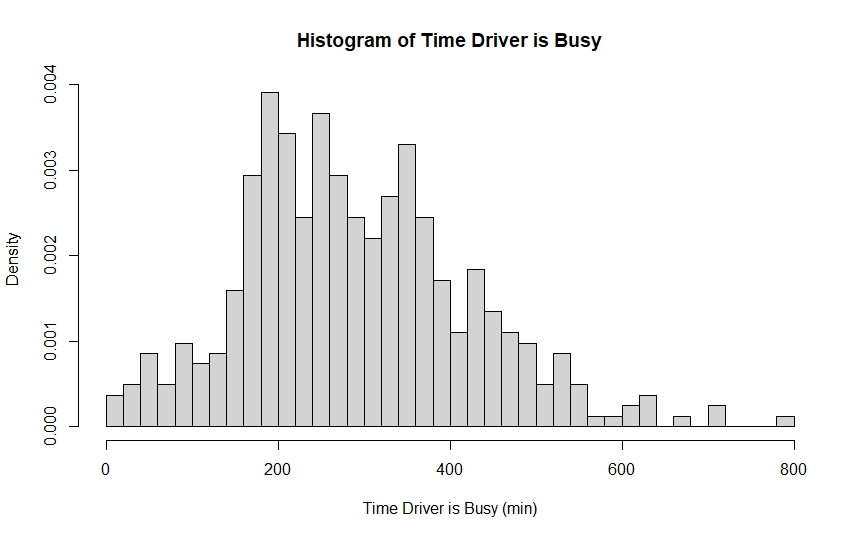
\includegraphics[scale=0.5]{isBusy_hist.jpeg}\\
\end{center}


We observed that this data seems to have the characteristics of a Normal distribution density. The following is a histogram with the normal distribution density fit without removal of values that can skew the parameters.
\begin{center}
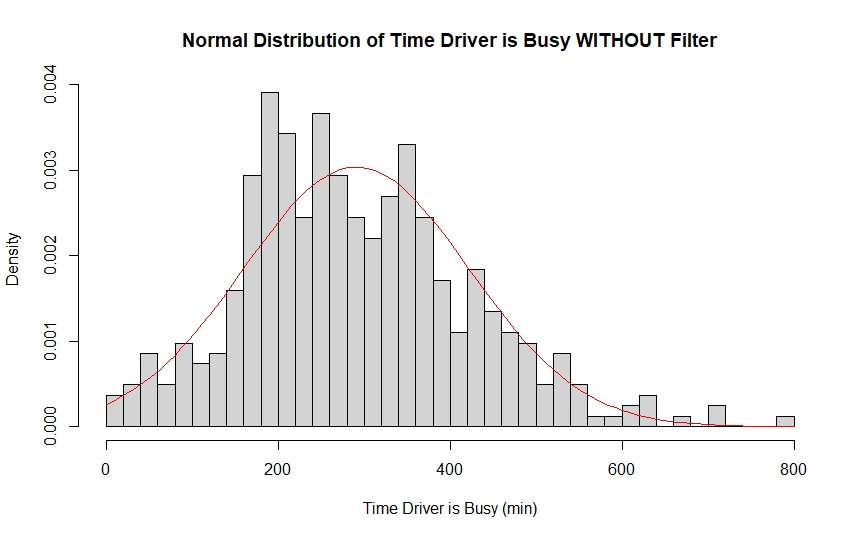
\includegraphics[scale=0.5]{isBusy_noFilter.jpeg} \\
\end{center}
\\
\\
The following is the result of cleaning the data such that it is within two standard deviations of the mean of the time a driver was busy.
\begin{center}
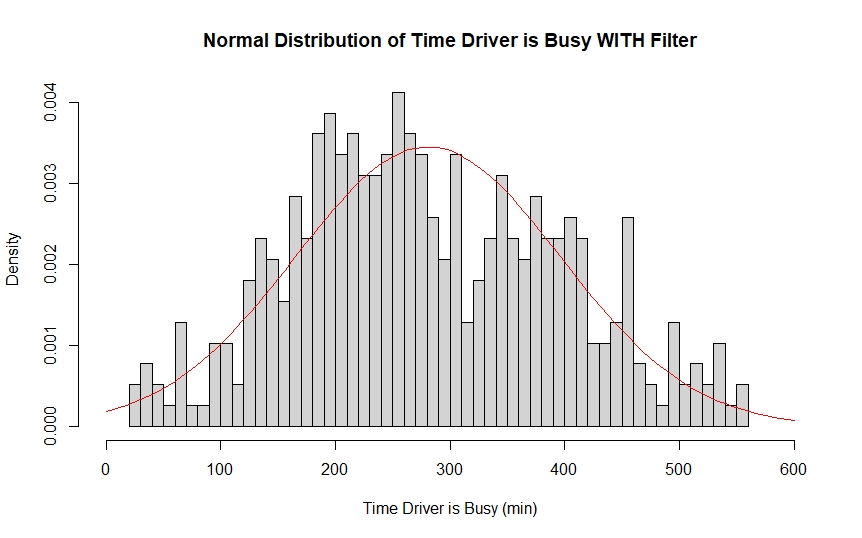
\includegraphics[scale=0.5]{isBusy_filtered2.jpeg}
\end{center}
\newpage
\subsection{Investigate whether the type of call used to summon the taxi makes much difference in mean trip time.}
In order to investigate if the call type is a influencing factor in the average trip time, we first took a sample of 10,000 from the supplied data set. Following the same logic as explained in 2.1 we removed the same values near zero and calculated trip duration as explained in section 2.1. Finally, we split each trip duration by call type and found the sample mean $\bar{X}$. In order to find the confidence interval for the true population constant for trip duration we found the upper and lower bound from our sample using the following formula:

\begin{equation}
    0.95 \approx P(\hat{\theta}-1.96\frac{\sigma}{\sqrt{n}} < \theta < \hat{\theta}+1.96\frac{\sigma}{\sqrt{n}} )
\end{equation}

Noting $\hat{\theta}$ is the sample approximation and $\theta$ is the true population constant

The following two graphs show the confidence intervals for A, B, and, C type calls:
\begin{center}
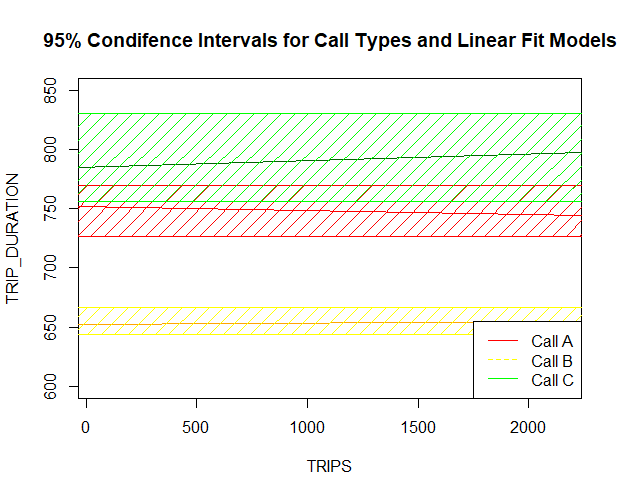
\includegraphics[scale=0.5]{95 Percent Confidence Intervals for Call Types and Linear Fit Models.png}    
\end{center}

\begin{center}
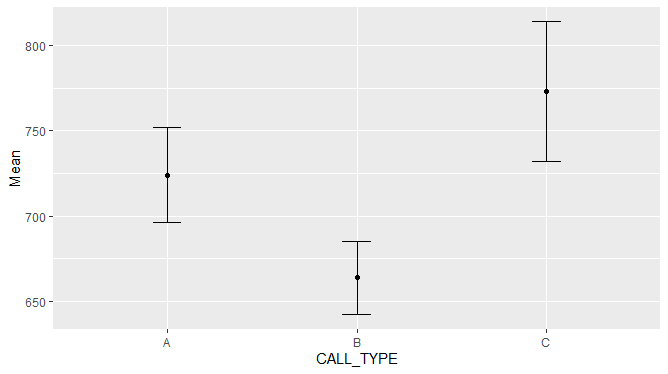
\includegraphics[scale=0.5]{MeanCallType_With95ConfidenceInterval.png}\\
\end{center}
\newpage

Additionally, the following represents the densities for each call type. As seen from the graph, each call type has roughly a similar shape distribution with different peaks with call type B having the largest peak followed by type A and lastly type C. 
\begin{center}
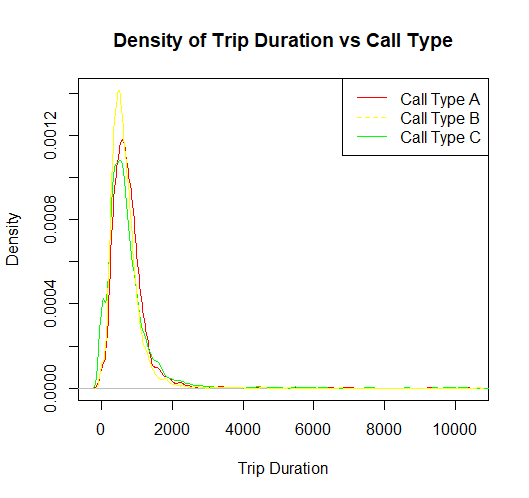
\includegraphics[scale=0.8]{Density_of_Trip_Duration_vs_Call_Type.png}\\    
\end{center}
The resulting confidence intervals of the mean time of all call type duration shows that A is about  $\approx$ sixty seconds greater than B, but $\approx$ sixty seconds less than C. Which leads us to believe the call type does on average have an effect on the average trip duration. Specifically, calls of type A (trips dispatched from central), type B (trips demanded to a taxi driver at a specific location) and type C (trips demanded from random streets). 

\subsection{Develop models for predicting trip time from other variables, both the explicit ones and also trip distance.}

\subsubsection{Linear Model}

The linear model to predict trip duration can be based on a variety of variables, including

\indent \text{TRIP DISTANCE}
\indent \text{CALL TYPE}
\indent \text{ORIGIN CALL}
\indent \text{ORIGIN STAND}
\indent \text{TAXI ID} ????

Staring with the TRIP DISTANCE, we can run a linear model using the following code once we have calculated both TRIP DURATION and TRIP DISTANCE from the polyline data.

\begin{lstlisting}
data <- train[, c("TRIP_DISTANCE", "TRIP_DURATION")]
fit <- lm(TRIP_DURATION ~ TRIP_DISTANCE, data)
# Using this linear fit, we can predict the TRIP_DURATION given the TRIP_DISTANCE of 1000 to 6000 in 1000 increments.
print(predict(fit, data.frame(TRIP_DISTANCE = c(1000, 2000, 3000, 4000, 5000, 6000)), interval = "confidence"))
\end{lstlisting}
Given a random sample of 10000 trained with the linear model, the code outputs.

\begin{verbatim}
       fit      lwr      upr
1 437.8944 424.6642 451.1246
2 499.5457 486.7629 512.3285
3 561.1970 548.7637 573.6302
4 622.8483 610.6582 635.0383
5 684.4995 672.4400 696.5591
6 746.1508 734.1054 758.1962
\end{verbatim}

which says that if the TRIP DISTANCE was 1000 meters, the TRIP DURATION would be around 437.9 seconds.

Next, to predict TRIP DURATION from CALL TYPE, the column of characters have to be changed into factors and indicator variables. Then we can do the linear model with this data as well, which can be used to predict the TRIP DURATION for call type A, B, and C as follows with a sample of 10000.
\begin{lstlisting}
train$CALL_TYPE <- as.factor(chunk1$CALL_TYPE)
train$CALL_A <- as.integer(as.integer(train$CALL_TYPE) == 1)
train$CALL_B <- as.integer(as.integer(train$CALL_TYPE) == 2)
train$CALL_C <- as.integer(as.integer(train$CALL_TYPE) == 3)

fit <- lm(TRIP_DURATION ~ CALL_B + CALL_C, train)
print(predict(fit, c(data.frame(CALL_B  = c(0,1,0)), data.frame(CALL_C  = c(0,0,1))), interval = "confidence"))
\end{lstlisting}  

\begin{verbatim}
       fit      lwr      upr
1 769.7324 740.2578 799.2069
2 666.1531 646.6066 685.6997
3 792.3341 767.9682 816.7000
\end{verbatim}
This tells us that the predicted TRIP DURATION for each type of call (which resembles the mean of those call type trip duration's pretty well).

If we were to combine these two into 1 linear model, we would get the following for TRIP DISTANCE of 3000 meters.
\begin{lstlisting}
 data <- chunk1[, c("TRIP_DURATION", "CALL_A", "CALL_B", "CALL_C", "TRIP_DISTANCE")]
 fit <- lm(TRIP_DURATION ~ CALL_B + CALL_C + TRIP_DISTANCE, data)
 print(predict(fit, c(data.frame(CALL_B  = c(0,1,0)), data.frame(CALL_C  = c(0,0,1)), data.frame(TRIP_DISTANCE  = c(3000, 3000, 3000))), interval = "confidence"))
\end{lstlisting}  
\begin{verbatim}
       fit      lwr      upr
1 591.1644 570.5055 611.8233
2 532.4805 518.4831 546.4779
3 565.9064 548.7747 583.0381
\end{verbatim}
This tells us that if the TRIP DISTANCE was 3000 meters, then the predicted TRIP DURATION would be these values for CALL TYPE A, B, and C.

To showcase how ORIGIN STAND and ORIGIN CALL might affect the TRIP DURATION, here is what a sample of 10000 gives.

\begin{lstlisting}
ogCall <- chunk1[!is.na(chunk1$ORIGIN_CALL),  c("TRIP_DURATION", "ORIGIN_CALL")]
fit <- lm(TRIP_DURATION ~ ORIGIN_CALL, ogCall)
print(predict(fit, data.frame(ORIGIN_CALL = c(10000, 30000, 50000, 100000)), interval = "confidence"))

ogStand <- chunk1[!is.na(chunk1$ORIGIN_STAND), c("TRIP_DURATION", "ORIGIN_STAND")]
fit <- lm(TRIP_DURATION ~ ORIGIN_STAND, ogStand)
print(predict(fit, data.frame(ORIGIN_STAND = c(5, 10, 15, 100)), interval = "confidence"))
\end{lstlisting}  
\begin{verbatim}
       fit      lwr      upr
1 762.3811 737.3351 787.4271
2 735.3263 714.0145 756.6382
3 708.2716 674.0685 742.4746
4 640.6347 557.8862 723.3832
       fit      lwr      upr
1 698.7655 673.5636 723.9674
2 693.7986 671.7978 715.7994
3 688.8316 669.6998 707.9634
4 604.3940 545.8918 662.8962
\end{verbatim}
This tells us that the linear model predicts that TRIP DURATION decreases as both ORIGIN CALL and ORIGIN STAND increases.

Finally, we can use all of these together to predict the TRIP DURATION for a trip that traveled 3000 meters, was call type B, and has the origin stand of 50.

\begin{lstlisting}
# Predict for DISTANCE = 3000, CALL TYPE = B, ORIGIN STAND = 50 (which already imples call type is B)
data <- chunk1[!is.na(chunk1$ORIGIN_STAND), c("TRIP_DURATION", "ORIGIN_STAND", "TRIP_DISTANCE")]
fit <- lm(TRIP_DURATION ~ ORIGIN_STAND + TRIP_DISTANCE, data)
print(predict(fit, c(data.frame(ORIGIN_STAND = 50), data.frame(TRIP_DISTANCE = 3000)), interval = "confidence"))
\end{lstlisting}  
\begin{verbatim}
       fit     lwr      upr
1 543.6792 530.372 556.9863
\end{verbatim}
From the code you can see we created a 95\% confidence interval with Y being the trip duration and U being the Origin Stand with a value of 50. \\

\boldsymbol{Linear \ Model \ Results} \\

Using the above linear model, we can form a regression function, this time with a sample of 100,000. 

\begin{equation}
    TRIP \ DURATION = \hat{\beta}_0 + \hat{\beta}_1 TRIP\textunderscore DURATION + \hat{\beta}_2 ORIGIN \textunderscore STAND + \hat{\beta}_3 TAXI \textunderscore ID \\
\end{equation}
\begin{equation}
    TRIP \ DURATION = -242100 + 0.05194t^{(1)} + -0.1262t^{(2)} + 0.01212t^{(3)}
\end{equation}

The detailed summary of the linear model is in Appendix A.4
Using our regression model, our mean absolute prediction error for the test set is 204.8012, which is around 3.4 minutes. Instead, what if we try to remove the TAXI ID from the model?

\begin{equation}
    TRIP \ DURATION = -242100 + 0.05194t^{(1)} + -0.1262t^{(2)}
\end{equation}
with the mean absolute prediction error of 200.8059, which is lower to around 3.35 minutes. Even when the TAXI ID is removed, there is little change in the error. 


We also created a polylinear model using distance and duration.
\begin{lstlisting}
data <- chunk1[, c("TRIP_DISTANCE", "TRIP_DURATION")]
predictionValue <- 100000
polyLinOut <- qePolyLin(data, "TRIP_DURATION", "ORIGN_CALL", "ORIGIN_STAND", "CALL_TYPE")
print(polyLinOut$testAcc)
print(predict(polyLinOut, predictionValue))
\end{lstlisting}
\begin{verbatim}
\end{verbatim}
Predicting trip distance and duration with polylinear model including the above variables was not giving us a usable result. We tried excluding various combinations of dummy variables but to no success. 

\newpage
\subsubsection{Machine Learning Models}


During our development of machine learning models we first attempted to predict trip duration with the k-nearest neighbor method. Using this method we can use trip distance, call type, origin call, and origin stand or any combination of the variables to predict the duration of a trip. First exploring fitting a model using trip distance we have the following code. 

\begin{lstlisting}
  data <- chunk1[, c("TRIP_DISTANCE", "TRIP_DURATION")]
  
  predictingVars <- c("TRIP_DISTANCE", "TRIP_DURATION")
  TnD <- chunk1[, predictingVars]

  predictionValue <- c(2000)
  
  print("KNN")
  kNNOut <- qeKNN(TnD, "TRIP_DURATION")
  print(kNNOut$testAcc)
  print(predict(kNNOut, predictionValue))
\end{lstlisting}  

With an input of the equivalent of two kilometers (line 6) it was predicted the duration would be 210.8178 seconds or roughly 3.5 minutes. However, the Mean Absolute Prediction Error on holdout set was 231.16363 seconds or roughly 3.8 minutes. So it seems the prediction error from the holdout set is less useful for smaller distances. Instead, using a distance of 15 kilometers yielded a prediction of 1476.6 seconds or 24 minutes plus or minus the same 3.8 minutes. 

% putttttttttt mixture of vars text

% ----------------------------------
Next using Random Forest we developed models for predicting trip time from the same variables used for k-nearest neighbor for later comparison. For random forest the code is nearly identical to create the model. However, for the same prediction variable (trip distance of 15 kilometers) we obtained a value of 1638.081 seconds (27.3 minutes) with a Mean Absolute Prediction Error of 254.0608 seconds (4.2 minutes). 
\\
% paragraph for a mixture of vars for Random forest

% ----------------------------


\newpage

For predicting trip duration based off of Origin stand and Origin call we used k nearest neighbors, random forests, and neural networks.  The following code accomplishes this task.
\begin{lstlisting}
  print("KNN")
  kNNOut <- qeKNN(ogCall, "TRIP_DURATION")
  print(kNNOut$testAcc)
  print(predict(kNNOut, 1000))

  print("KNN")
  kNNOut <- qeKNN(ogStand, "TRIP_DURATION")
  print(kNNOut$testAcc)
  print(predict(kNNOut, 100))
  
  print("RF")
  rfOut <- qeRF(ogCall, "TRIP_DURATION")
  print(rfOut$testAcc)
  print(predict(rfOut, 1000))
  
  print("RF")
  rfOut <- qeRF(ogStand, "TRIP_DURATION")
  print(rfOut$testAcc)
  print(predict(rfOut, 100))
  
  print("Neural")
  neuralOut <- qeNeural(ogCall, "TRIP_DURATION")
  print(neuralOut$testAcc)
  print(predict(neuralOut, 1000))
  
  print("Neural")
  neuralOut <- qeNeural(ogStand, "TRIP_DURATION")
  print(neuralOut$testAcc)
  print(predict(neuralOut, 100))
\end{lstlisting}

Prediction of trip duration results of above code in seconds 
\begin{verbatim}
                      KNN        RF            Neural
 Origin Call          747     613.8851       853.6945
Origin Stand          745.2   702.2723       258.0748
 
\end{verbatim}

We also have the following accuracy's in seconds associated with each ML prediction type.  
\begin{verbatim}
                      KNN        RF            Neural
 Origin Call        345.3634   352.7744       398.9556
Origin Stand        305.3667   314.0336       316.7653
 
\end{verbatim}

Clearly in this case the best prediction method based on both origin call and origin stand is using k nearest neighbors as its mean average prediction error is the lowest.

\newpage 

\subsubsection{Comparing Models}

\begin{verbatim}
    qeFtn   meanAcc
1 qePolyLin 278.2424
2 qeKNN 231.1636
3 qeNeural 309.0910
4 qeRF 246.3505
\end{verbatim}

\begin{lstlisting}
# This will compare the machine learning and linear models in predicting TRIP_DURATION
TnD <- chunk1[, c("TRIP_DISTANCE", "TRIP_DURATION", "TAXI_ID", "TIMESTAMP")]
print(qeCompare(TnD,'TRIP_DURATION', c('qePolyLin','qeKNN', 'qeNeural', 'qeRF', 'qeGBoost'), 15))
\end{lstlisting}

\begin{lstlisting}
  # Predicting from TRIP DISTANCE, ORIGIN STAND, and technically CALL TYPE
  data <- chunk1[!is.na(chunk1$ORIGIN_STAND), c("TRIP_DURATION", "TRIP_DISTANCE", "ORIGIN_STAND")]
  # Filter by rows with ORIGN STAND value, which means that CALL TYPE will always be B. 
  predictionValue <- c(3000, 5)
  
   mlFit <- qeKNN(data, "TRIP_DURATION")
  print(predict(mlFit, predictionValue))
  
  mlFit <- qeRF(data, "TRIP_DURATION")
  print(predict(mlFit, predictionValue))
  
  mlFit <- qeNeural(data, "TRIP_DURATION")
  print(predict(mlFit, predictionValue))
  
  mlFit <- qeGBoost(data, "TRIP_DURATION")
  print(predict(mlFit, predictionValue))
  
  print(qeCompare(data,'TRIP_DURATION', c('qePolyLin','qeKNN', 'qeNeural', 'qeRF', 'qeGBoost'), 10))
  print(MAPE(lm(TRIP_DURATION ~ TRIP_DISTANCE + ORIGIN_STAND, data)$fitted.values, data$TRIP_DURATION))
  
\end{lstlisting}

\begin{verbatim}
      qeFtn  meanAcc
1 qePolyLin 250.1575
2     qeKNN 182.8530
3  qeNeural 276.5464
4      qeRF 188.3985
5  qeGBoost 196.0283
[1] 194.7717
\end{verbatim}

Running 10 iterations of the different machine learning and linear models, it tells us that K Nearest Neighbors and Random Forest have the best accuracy able to predict with an error of 182-188 seconds or just around 3 minutes.

However, in when looking at the confidence intervals with the TRIP DURATION of the \textit{sample} data, we see that an error of 180 seconds is quite a lot.
\begin{lstlisting}
t.test(chunk1$TRIP_DURATION)    
\end{lstlisting}
\begin{verbatim}
95 percent confidence interval:
 707.5583 733.6598
sample estimates:
mean of x 
 720.6091    
\end{verbatim}

This says that the 95 percent confidence interval only has a range of around 26 seconds, which means that the linear and machine learning methods are not very useful in predicting the TRIP DURATION in this situation with this sample size. Nonetheless, KNN performed the best with the given information.


\section{Contributions}

\subsection{Rohan Skariah}
\begin{itemize}
    \item Let T denote trip duration. Explore finding a model for $fT$ from one of our density families.
    \begin{itemize}
        \item Derived trip duration from GPS data using cited code
        \item Discussed possible method of fitting ditributions with group
    \end{itemize}
    \item Let B denote the proportion of time a driver is busy, i.e. actually driving rather than waiting for the next fare. Explore finding a model for $f_B$ from one of our density families.
    \begin{itemize}
        \item Debugged teammates code and provided solution to sum driver busy time from GPS data and timestamps
        \item Cleaned data in order to better fit a Normal Distribution to the histogram of busy time
    \end{itemize}
    \item Investigate whether the type of call used to summon the taxi makes much difference in mean trip time.
      \begin{itemize}
        \item Provided code that separated data by call type and calculated individual confidence intervals
        \item Visualized confidence interval in three different ways
        \item Provided a density graph for different call types and trip duration to visualize differences in density by call type
    \end{itemize}
    \item Develop models for predicting trip time from other variables, both the explicit ones and also trip distance.
     \begin{itemize}
        \item Wrote code to isolate data needed for creating a variety of models such as KNN, RF, and Neural.
        \item Fit ordinary linear model to data
        \item Provided code that helped in distinguishing which machine learning models were preforming best
        \item Developed model for trip duration with multiple predictor variables
        
    \end{itemize}
    
\end{itemize}


\subsection{Nathan Krieger}
\begin{itemize}
\item Assisted other members in installing regtools and troubleshooting other dependency issues
 \item Find a density for trip duration
  \begin{itemize}
    \item Visualized trip duration data with histogram and various curves
    \item Compared a variety of method for parameter estimation such as MLE and MM
    \item Removed inaccurate values from data that skewed parameter estimation
   \end{itemize}
   
  \item Let B denote the proportion of time a driver is busy, i.e. actually driving rather than waiting for the next fare. Explore finding a model for fB from one of our density families.
    \begin{itemize}
     \item Assisted in fitting an approximately normal graph  
     \item Assisted in wording for tex section and graph/histogram creation
   \end{itemize}
  \item Investigate whether the type of call used to summon the taxi makes much difference in mean trip time.
    \begin{itemize}
     \item Wrote up tex file section, positioned graphs, included formulas, and provided explanations of findings
   \end{itemize}
  \item Develop models for predicting trip time from other variables, both the explicit ones and also trip distance. 
    \begin{itemize}
     \item Developed,executed, and interpreted results from machine learning models for qeKNN() and qeRF() for predicting trip duration from trip distance specifically
     \item Wrote tex file for Machine learning models section 
    \end{itemize}

\end{itemize}
\subsection{Raymond Laughrey}
\begin{itemize}
    \item Explored method of moments and Maximum likelihood Estimation for finding a model of trip duration density. 
    \item Conferred with Geoff about finding a model for density of trip time a driver is busy.
    \item Found difference in mean trip time based on type of call used to summon taxi.
    \begin{itemize}
        \item Created bar graph visualizing call type mean and confidence intervals.
    \end{itemize}
    \item Explored qePolyLin when developing trip time prediction from other variables. 
    \item Used quCompare to find differences in various ML models.

\end{itemize}

\subsection{Geoffrey Cook}
\begin{itemize}
    \item Installed regtools and assisted other group members
    \item Was able to read the train.csv file and assisted other group members
    \item Found that trip duration density fit a gamma distribution after testing a couple different families, group agreed.
    \item Removed trip duration's that were less than one minute. Group decided to only remove trips that were less than 15 seconds
    \item Made the trip duration's histogram and was able to fit a curve to it.
    \item Used iterative estimation to get the best gamma density curve fit, but we agreed it probably wasn't best to use my method despite the fact it worked with random samples of various sizes.
    \item Found start time and end time of trips and was able to convert from UNIX to actual dates and times.  We did not end up needing this.
    \item Coded and wrote the LaTex for the proportion of time a driver is busy, with Rohan assisting in the R code to figure out how to add trip durations.  Upon his suggestion we removed outlier data that was not within two standard deviations.
    \item Coded and wrote the LaTex for using machine learning models for predicting trip duration based off origin stand and origin call.
    \item Assisted the group in understanding that accuracy values were in seconds and 200 was not an absurd amount.  Although the confidence intervals did not appear to reflect this.  Double checked the confidence intervals and prediction accuracy data up to a random sample of 300k.
    \item Commented code and helped to remove some functions that ended up being unnecessary.
\end{itemize}




\appendix{} \section{Appendix}

\subsection{Executing the Code}
\begin{lstlisting}
  # Set the working directory and load in the train data as you see fit.
# setwd("D:/UC Davis/Computer Science/ECS 132/Term Project")
# train <- read.csv('../train.csv')

# Libraries used
library(regtools)
library(datetime)
library(rjson)
library(data.table)
library(randomForest)
library(gbm)
library(keras)
library(glmnet)
library(tensorflow)
library(ggplot2)
library(rcompanion)
library(ggmap)

# Sample size for data calculations
numRowsToCalculate <- 10000

cat("Rows Calculated:", numRowsToCalculate, "\n")

# Sample the data or take the fist 'numRowsToCalculate' rows from the csv itself.
chunk1 <- train[sample(nrow(train), numRowsToCalculate), ]
#chunk1 <- read.csv(file = "../train.csv", nrows = numRowsToCalculate)

# Analyze and populate TRIP_DURATION, TRIP_DISTANCE, CALL_A, CALL_B, CALL_C, DAY_A, DAY_B, DAY_C
chunk1 <- AnalyzeInitialData(chunk1)

clean <- TRUE
minDur <- 15
maxDur <- 10000
cleanData()

CalculateBusyTime()
plotMeanDurationByCallType()

plotDurationByCallType()
confidenceIntervalCallTypes()

linearModel()
comparingNeural()
machineLearningModel()
originCallandStandAndML()
\end{lstlisting}

\subsection{Code: Analyzing the Data and Populating Columns} 
\begin{lstlisting}
AnalyzeInitialData <- function(chunk1) {
  trip_durations <- c()
  trip_distance <- c()

  chunk1 <- chunk1[as.logical(chunk1$MISSING_DATA) == FALSE, ]
  
  # Get TRIP DISTANCE and TRIP DURATION from POLYLINE chunk1#
  for (i in 1:nrow(chunk1)) {
    distance_sum <- 0
    lonlat <- fromJSON(chunk1$POLYLINE[i])
    
    len <- length(lonlat)
    if (len > 1) {
      for (j in 1:(len - 1)) {
        distance_sum <- distance_sum + HaversineDistance(lonlat[[j]][2], lonlat[[j]][1], lonlat[[j+1]][2], lonlat[[j+1]][1])
      }
    } else distance_sum <- 0
    trip_durations <- append(trip_durations, (len - 1) * 15) # Calculated in seconds
    trip_distance <- append(trip_distance, distance_sum) # Calculated in meters
  }
  chunk1 <- cbind(chunk1, TRIP_DURATION=trip_durations)
  chunk1 <- cbind(chunk1, TRIP_DISTANCE=trip_distance)
  
  # Plot the histogram if you see fit
  # hist(chunk1$TRIP_DISTANCE, breaks = 100, freq = FALSE, xlim = c(0, 50000))
  # hist(chunk1$TRIP_DURATION, breaks = 100, freq = FALSE, xlim = c(0, 5000))
  
  # Seperate CALL TYPES into indicator variables #
  chunk1$CALL_TYPE <- as.factor(chunk1$CALL_TYPE)
  chunk1$CALL_A <- as.integer(as.integer(chunk1$CALL_TYPE) == 1)
  chunk1$CALL_B <- as.integer(as.integer(chunk1$CALL_TYPE) == 2)
  chunk1$CALL_C <- as.integer(as.integer(chunk1$CALL_TYPE) == 3)
  
  # Seperate DAY TYPES into indicator variables #
  ## NOTE: with correct data, this will be useful, not in this case because this column was calculated incorrectly ##
  chunk1$DAY_TYPE <- as.factor(chunk1$DAY_TYPE)
  chunk1$DAY_A <- as.integer(as.integer(chunk1$DAY_TYPE) == 1)
  chunk1$DAY_B <- as.integer(as.integer(chunk1$DAY_TYPE) == 2)
  chunk1$DAY_C <- as.integer(as.integer(chunk1$DAY_TYPE) == 3)
  
  print("TRIP DISTANCE")
  print(summary(chunk1$TRIP_DISTANCE))
  print("TRIP DURATION")
  print(summary(chunk1$TRIP_DURATION))
  print("CALL A")
  print(summary(chunk1$CALL_A))
  print("CALL B")
  print(summary(chunk1$CALL_B))
  print("CALL C")
  print(summary(chunk1$CALL_C))
  print("DAY A")
  print(summary(chunk1$DAY_A))
  print("DAY B")
  print(summary(chunk1$DAY_B))
  print("DAY C")
  print(summary(chunk1$DAY_C))
  
  return (chunk1)
}
\end{lstlisting}
The output graphs for this code is in section 2.6.
\begin{verbatim}
Rows Calculated: 10000 
[1] "TRIP DISTANCE"
   Min. 1st Qu.  Median    Mean 3rd Qu.    Max. 
      0    2416    3976    5385    6489   87970 
[1] "TRIP DURATION"
   Min. 1st Qu.  Median    Mean 3rd Qu.    Max. 
  -15.0   405.0   600.0   716.2   870.0 32610.0 
[1] "CALL A"
   Min. 1st Qu.  Median    Mean 3rd Qu.    Max. 
 0.0000  0.0000  0.0000  0.2174  0.0000  1.0000 
[1] "CALL B"
   Min. 1st Qu.  Median    Mean 3rd Qu.    Max. 
 0.0000  0.0000  0.0000  0.4716  1.0000  1.0000 
[1] "CALL C"
   Min. 1st Qu.  Median    Mean 3rd Qu.    Max. 
  0.000   0.000   0.000   0.311   1.000   1.000 
[1] "DAY A"
   Min. 1st Qu.  Median    Mean 3rd Qu.    Max. 
      1       1       1       1       1       1 
[1] "DAY B"
   Min. 1st Qu.  Median    Mean 3rd Qu.    Max. 
      0       0       0       0       0       0 
[1] "DAY C"
   Min. 1st Qu.  Median    Mean 3rd Qu.    Max. 
      0       0       0       0       0       0
\end{verbatim}

\subsection{Code: HaversineDistance}
\begin{lstlisting}
HaversineDistance <- function(lat1, lon1, lat2, lon2) {
  # This function was taken from online
  # https://github.com/santiagomota/kaggle-taxi-II/blob/master/taxi.R
  # returns the distance in m
  REarth <- 6378137
  lat  <- abs(lat1-lat2)*pi/180
  lon  <- abs(lon1-lon2)*pi/180
  lat1 <- lat1*pi/180
  lat2 <- lat2*pi/180
  a    <- sin(lat/2)*sin(lat/2)+cos(lat1)*cos(lat2)*sin(lon/2)*sin(lon/2)
  d    <- 2*atan2(sqrt(a), sqrt(1-a))
  d    <- REarth*d
  return(d)
}
\end{lstlisting}

\subsection{Code: Clean Data}
\begin{lstlisting}
clean <- TRUE
minDur <- 15 #seconds
maxDur <- 10000 #seconds
cleanData()

cleanData <- function() {
  if (clean) {
    chunk1 <- chunk1[chunk1$TRIP_DURATION < maxDur,]
    chunk1 <- chunk1[chunk1$TRIP_DURATION > minDur,]
    chunk1 <- chunk1[as.logical(chunk1$MISSING_DATA) == FALSE, ]
  }
}
\end{lstlisting}

\subsection{Code: Plotting Mean Trip Duration by Call Type} 

\begin{lstlisting}
plotMeanDurationByCallType <- function() {
  library(ggplot2)
  chunk1$CALL_TYPE <- as.factor(chunk1$CALL_TYPE)
  Sum = groupwiseMean(TRIP_DURATION ~ CALL_TYPE,
                      data   = chunk1,
                      conf   = 0.95,
                      digits = 3)
  print(Sum)
  
  qplot(x = CALL_TYPE, y = Mean, data = Sum) +
  geom_errorbar(aes(ymin = Trad.lower, ymax  = Trad.upper, width = 0.15))
}  
\end{lstlisting}
The image produced from this code is included in Section 2.7 
\begin{verbatim}
  CALL_TYPE    n Mean Conf.level Trad.lower Trad.upper
1         A 2169  731       0.95        712        749
2         B 4763  669       0.95        652        685
3         C 3068  778       0.95        745        812    
\end{verbatim}

\subsection{Code: Visualization of Trip Duration by Call Type using Linear Regression} 
\begin{lstlisting}
confidenceIntervalCallTypes <- function() { 
  chunk1$CALL_TYPE <- as.factor(chunk1$CALL_TYPE)
  
  call_A_Duration <- chunk1[(as.integer(chunk1$CALL_TYPE) == 1), c("TRIP_DURATION")]
  call_B_Duration <- chunk1[(as.integer(chunk1$CALL_TYPE) == 2), c("TRIP_DURATION")]
  call_C_Duration <- chunk1[(as.integer(chunk1$CALL_TYPE) == 3), c("TRIP_DURATION")]
  
  conf_95_A <- t.test(call_A_Duration)$conf.int
  conf_95_B <- t.test(call_B_Duration)$conf.int
  conf_95_C <- t.test(call_C_Duration)$conf.int

  xlimVal <- min(length(call_A_Duration), length(call_B_Duration), length(call_C_Duration))
  plot(1, main = "95% Condifence Intervals for Call Types and Linear Fit Models", xlab = "TRIPS", ylab = "TRIP_DURATION", xlim = c(50,xlimVal), ylim = c(600, 850))
  
  abline(lm(call_A_Duration~c(1:length(call_A_Duration))), col="red")
  abline(lm(call_B_Duration~c(1:length(call_B_Duration))), col="orange")
  abline(lm(call_C_Duration~c(1:length(call_C_Duration))), col="darkgreen")
  
  densVal <- 10
  rect(-100, conf_95_A[1], xlimVal + 100, conf_95_A[2], density = densVal, col = "red")
  rect(-100, conf_95_B[1], xlimVal + 100, conf_95_B[2], density = densVal, col = "yellow")
  rect(-100, conf_95_C[1], xlimVal + 100, conf_95_C[2], density = densVal, col = "green")
  legend("bottomright", lty=c(1,2,1,2), legend = c("Call A", "Call B", "Call C"), col = c("red", "yellow", "green"))
}
\end{lstlisting}
The image produced from this code is included in Section 2.7.

\subsection{Code: Plotting Trip Duration Density By Call Type} 
\begin{lstlisting}
plotDurationByCallType <- function() {
  a <- density(chunk1[chunk1$CALL_A == 1, c("TRIP_DURATION")]) # returns the density data
  b <- density(chunk1[chunk1$CALL_B == 1, c("TRIP_DURATION")]) # returns the density data
  c <- density(chunk1[chunk1$CALL_C == 1, c("TRIP_DURATION")]) # returns the density data
  
  max_val <- max(max(a$y), max(b$y), max(c$y))
  plot(a, col = "red", ylim=c(0,max_val), xlab="Trip Duration", main="Density of Trip Duration vs Call Type") # plots the results
  lines(c, col = "green") 
  lines(b, col = "yellow") 
  legend("topright", lty=c(1,2,1,2), legend = c("Call Type A", "Call Type B", "Call Type C"), col = c("red", "yellow", "green"))
}
\end{lstlisting}

\subsection{Code: Calculating Time Driver is Busy and Waiting} 
\begin{lstlisting}
CalculateBusyTime <- function() {
  #Calculates the time a driver is busy
  chunk2 <- train[1:numRowsToCalculate,5:9]
  
  trip_durations_chunk2 <- c()
  finish_time <- c()
  for (i in 1:nrow(chunk2)) {
    polyline_data <- as.list(strsplit(chunk1[[9]][i], "],")[[1]])
    polyline_data <- gsub("[[]", "", polyline_data)
    trip_durations_chunk2 <- append(trip_durations_chunk2, (length(polyline_data) - 1) * 15) # 
  }
  finish_time <- append(finish_time, chunk2$TIMESTAMP + trip_durations_chunk2)
  
  #Add columns for trip duration and trip finish time
  chunk2 <- cbind(chunk2, TRIP_DURATION=trip_durations_chunk2)
  chunk2 <- cbind(chunk2, FINISH_TIME=finish_time)
  #Was used to convert UNIX timestamp but realized we don't need to do that
  # chunk2$TIMESTAMP <- as.POSIXct(chunk2$TIMESTAMP, origin="1970-01-01")
  # FINISH_TIME <- as.POSIXct(chunk2$FINISH_TIME, origin="1970-01-01")
  
  #Removes trips that were not greater than 15 seconds and splits them by taxi id
  chunk2 <- chunk2[!(chunk2$TRIP_DURATION <= "15"), ]
  is_busy <- chunk2[,c("TAXI_ID", "TIMESTAMP", "TRIP_DURATION" , "FINISH_TIME" )]
  split_by_id <- split(is_busy, is_busy$TAXI_ID)
  
  driverWaiting <- c()
  driverBusy <- c()
  
  #Calculates the time a driver is busy as well as the time a driver is not busy
  for (i in 1:length(split_by_id)) {
    sumDuration <- 0
    for (j in 1:length(split_by_id[[i]]$TRIP_DURATION))
      sumDuration <- sumDuration + split_by_id[[i]]$TRIP_DURATION[j]
    timeDifference <- (split_by_id[[i]]$TIMESTAMP[length(split_by_id[[i]]$TIMESTAMP)] - split_by_id[[i]]$TIMESTAMP[1])
    driverWaiting <- append(driverWaiting, (timeDifference - sumDuration))
    driverBusy <- append(driverBusy, sumDuration)
    
  }
  #Histogram for time a driver is not busy
  hist(driverWaiting, breaks = 100, freq = FALSE)
  
  #Histogram for time a driver is busy
  hist(driverBusy, breaks = 50, freq = FALSE, main = "Normal Distribution of Time Driver is Busy WITHOUT Filter", xlab = "Time Driver is Busy in Seconds")
  curve(dnorm(x, mean = mean(driverBusy), sd = sd(driverBusy)), col = "red", add = TRUE)
  
  #Cleaning the data by removing anything that is not within two standard deviations
  std2 <- 2 * sd(driverBusy)
  meanBusy <- mean(driverBusy)
  driverBusy <- driverBusy[driverBusy > (meanBusy - std2)]
  driverBusy <- driverBusy[driverBusy < (meanBusy + std2)]
  
  #Histogram for time a driver is busy with data cleaned
  hist(driverBusy, breaks = 50, freq = FALSE, main = "Normal Distribution of Time Driver is Busy WITH Filter", xlab = "Time Driver is Busy in Seconds")
  curve(dnorm(x, mean = mean(driverBusy), sd = sd(driverBusy)), col = "red", add = TRUE)
  
  print(mean(driverBusy))
  print(sd(driverBusy))
  print(mean(driverWaiting))
  print(sd(driverWaiting))
}
\end{lstlisting}
\begin{verbatim}
Rows Calculated: 10000 
[1] 13300.23
[1] 5732.898
[1] 134573.3
[1] 37918.31
\end{verbatim}

\subsection{Code: Linear Model} 
\begin{lstlisting}
linearModel <- function() {
  data <- chunk1[, c("TRIP_DISTANCE", "TRIP_DURATION")]
  # Using this linear fit, we can predict the TRIP_DURATION given the TRIP_DISTANCE of 1000 to 6000 in 1000 increments.
  fit <- lm(TRIP_DURATION ~ TRIP_DISTANCE, data)
  print(predict(fit, data.frame(TRIP_DISTANCE = c(1000, 2000, 3000, 4000, 5000, 6000)), interval = "confidence"))
  
  data <- chunk1[, c("TRIP_DURATION", "CALL_A", "CALL_B", "CALL_C")]
  fit <- lm(TRIP_DURATION ~ CALL_B + CALL_C, data)
  print(predict(fit, c(data.frame(CALL_B  = c(0,1,0)), data.frame(CALL_C  = c(0,0,1))), interval = "confidence"))
  
  data <- chunk1[, c("TRIP_DURATION", "CALL_A", "CALL_B", "CALL_C", "TRIP_DISTANCE")]
  fit <- lm(TRIP_DURATION ~ CALL_B + CALL_C + TRIP_DISTANCE, data)
  print(predict(fit, c(data.frame(CALL_B  = c(0,1,0)), data.frame(CALL_C  = c(0,0,1)), data.frame(TRIP_DISTANCE  = c(3000, 3000, 3000))), interval = "confidence"))
  
  ogCall <- chunk1[!is.na(chunk1$ORIGIN_CALL),  c("TRIP_DURATION", "ORIGIN_CALL")]
  fit <- lm(TRIP_DURATION ~ ORIGIN_CALL, ogCall)
  print(predict(fit, data.frame(ORIGIN_CALL = c(10000, 30000, 50000, 100000)), interval = "confidence"))
  
  ogStand <- chunk1[!is.na(chunk1$ORIGIN_STAND), c("TRIP_DURATION", "ORIGIN_STAND")]
  fit <- lm(TRIP_DURATION ~ ORIGIN_STAND, ogStand)
  print(predict(fit, data.frame(ORIGIN_STAND = c(5, 10, 15, 100)), interval = "confidence"))
  
  # Predict for DISTANCE = 3000, CALL TYPE = B, ORIGIN STAND = 50 (which already imples call type is B)
  data <- chunk1[!is.na(chunk1$ORIGIN_STAND), c("TRIP_DURATION", "TRIP_DISTANCE", "ORIGIN_STAND", "TAXI_ID")]
  fit <- lm(TRIP_DURATION ~ TRIP_DISTANCE + ORIGIN_STAND + TAXI_ID, data)
  print(summary(fit))
  print(MAPE(fit$fitted.values, data$TRIP_DURATION))
  
  data <- chunk1[!is.na(chunk1$ORIGIN_STAND), c("TRIP_DURATION", "TRIP_DISTANCE", "ORIGIN_STAND")]
  fit <- lm(TRIP_DURATION ~ TRIP_DISTANCE + ORIGIN_STAND, data)
  print(summary(fit))
  print(MAPE(fit$fitted.values, data$TRIP_DURATION))
  
  data <- chunk1[, c("TRIP_DURATION", "TRIP_DISTANCE")]
  data$TRIP_DURATION <- data$TRIP_DURATION
  print("lm")
  fit <- lm(TRIP_DURATION ~ TRIP_DISTANCE, data)
  print(summary(fit))
  print(MAPE(fit$fitted.values, data$TRIP_DURATION))
  
  data <- chunk1[!is.na(chunk1$CALL_A), c("TRIP_DISTANCE", "TRIP_DURATION", "CALL_A")]
  predictionValue <- c(3000,0)
  print("PolyLin")
  qePolyLinOut <- qePolyLin(data,"TRIP_DURATION")
  print(qePolyLinOut$testAcc)
}
\end{lstlisting}

\subsection{Code: Machine Learning Models} 
\begin{lstlisting}
machineLearningModel <- function() {
  data  <- chunk1[, c("TRIP_DISTANCE", "TRIP_DURATION")]
  predictingVars  <- c("TRIP_DISTANCE", "TRIP_DURATION")
  TnD  <- chunk1[, predictingVars]
  predictionValue  <- c(2000)
  print("KNN")
  kNNOut  <- qeKNN(TnD , "TRIP_DURATION")
  print(kNNOut$testAcc)
  print(predict(kNNOut , predictionValue))

  data <- chunk1[, c("TRIP_DURATION", "TRIP_DISTANCE", "CALL_A", "CALL_B", "CALL_C")]

  # Predicting from TRIP DISTANCE, ORIGIN STAND, and technically CALL TYPE
  data <- chunk1[!is.na(chunk1$ORIGIN_STAND), c("TRIP_DURATION", "TRIP_DISTANCE", "ORIGIN_STAND")]
  predictionValue <- c(5000, 10)

  mlFit <- qePolyLin(data, "TRIP_DURATION")
  print(mlFit$testAcc)

  mlFit <- qeKNN(data, "TRIP_DURATION")
  print(mlFit$testAcc)
  print(predict(mlFit, predictionValue))

  mlFit <- qeRF(data, "TRIP_DURATION")
  print(mlFit$testAcc)
  print(predict(mlFit, predictionValue))

  mlFit <- qeNeural(data, "TRIP_DURATION")
  print(mlFit$testAcc)
  print(predict(mlFit, predictionValue))

  mlFit <- qeGBoost(data, "TRIP_DURATION")
  print(mlFit$testAcc)
  print(predict(mlFit, predictionValue))

  print(qeCompare(data,'TRIP_DURATION', c('qePolyLin','qeKNN', 'qeNeural', 'qeRF', 'qeGBoost'), 10))
  print(MAPE(lm(TRIP_DURATION ~ TRIP_DISTANCE + ORIGIN_STAND, data)$fitted.values, data$TRIP_DURATION))
  data <- chunk1[!is.na(chunk1$ORIGIN_CALL), c("TRIP_DURATION", "TRIP_DISTANCE", "CALL_A", "CALL_B", "CALL_C", "ORIGIN_CALL")]

  fit <- qePolyLin(data, "TRIP_DURATION")
  print(fit$testAcc)

  data <- chunk1[, c("TRIP_DISTANCE", "TRIP_DURATION")]
  print(qeCompare(data,'TRIP_DURATION', c('qePolyLin','qeKNN', 'qeNeural', 'qeRF'), 10))

  predictionValue <- 5500
  print("KNN")
  kNNOut <- qeKNN(data, "TRIP_DURATION")
  print(kNNOut$testAcc)
  print(predict(kNNOut, predictionValue))

  print("PolyLin")
  polyLinOut <- qePolyLin(data, "TRIP_DURATION")
  print(polyLinOut$testAcc)
  print(predict(polyLinOut, predictionValue))

  print("RF")
  rFOut <- qeRF(data, "TRIP_DURATION")
  print(rFOut$testAcc)
  print(predict(rFOut, predictionValue))

  print("Neural")
  neuralOut <- qeNeural(data, "TRIP_DURATION")
  print(neuralOut$testAcc)
  print(predict(neuralOut, predictionValue))
  
  data <- chunk1[, c("TRIP_DISTANCE", "CALL_A", "CALL_B", "CALL_C", "TRIP_DURATION")]
  predictionValue <- c(3000, 0, 1, 0)
  
  print("gBoost")
  gBoostOut <- qeGBoost(data, "TRIP_DURATION")
  print(gBoostOut$testAcc)
  print(predict(gBoostOut, predictionValue))
  
  print(qeCompare(data,'TRIP_DURATION', c('qePolyLin','qeKNN', 'qeNeural', 'qeRF', 'qeGBoost'), 10))
}
\end{lstlisting}

\subsection{Code: Non default Hyper Parameters for qeNeural machine learning model}
\begin{lstlisting}
comparingNeural <- function() {
  ### Testing non default hyperparameters for qeNeural ##

  # Trying  to find  which  hyper  parameters  work  best  for  qeNeural.
  data  <- chunk1[!is.na(chunk1$ORIGIN_STAND), c("TRIP_DURATION", "TRIP_DISTANCE", "ORIGIN_STAND")]
  predictionValue <- c(3000, 50)
  
  mlFit1 <- qeNeural(data, "TRIP_DURATION")
  mlFit2 <- qeNeural(data, "TRIP_DURATION",nEpoch=10)
  mlFit3 <- qeNeural(data, "TRIP_DURATION",nEpoch=50)
  mlFit4 <- qeNeural(data, "TRIP_DURATION", hidden = c(50, 50))
  mlFit5 <- qeNeural(data, "TRIP_DURATION", hidden = c(500, 500))
  mlFit6 <- qeNeural(data, "TRIP_DURATION", hidden = c(1000, 1000))
  
  print(mlFit1$testAcc)
  #print(predict(mlFit1, predictionValue))
  print(mlFit2$testAcc)
  #print(predict(mlFit2, predictionValue))
  print(mlFit3$testAcc)
  #print(predict(mlFit3, predictionValue))
  print(mlFit4$testAcc)
  #print(predict(mlFit4, predictionValue))
  print(mlFit5$testAcc)
  #print(predict(mlFit5, predictionValue))
  print(mlFit6$testAcc) # <-- Most accurate
  #print(predict(mlFit6, predictionValue)) 
})
\end{lstlisting}
\begin{verbatim}
[1] 191.3562
[1] 233.1253
[1] 223.6629
[1] 219.7309
[1] 217.3234
[1] 179.6353
\end{verbatim}

\subsection{Results: Linear Model for TRIP DURATION}
\begin{verbatim}
Call:
lm(formula = TRIP_DURATION ~ TRIP_DISTANCE + ORIGIN_STAND + TAXI_ID, 
    data = data)

Residuals:
     Min       1Q   Median       3Q      Max 
-17527.8   -177.8    -59.9    104.6  25116.4 

Coefficients:
                Estimate Std. Error t value Pr(>|t|)    
(Intercept)   -2.421e+05  1.580e+05  -1.532    0.126    
TRIP_DISTANCE  5.194e-02  2.638e-04 196.861   <2e-16 ***
ORIGIN_STAND  -1.262e-01  9.448e-02  -1.336    0.182    
TAXI_ID        1.212e-02  7.901e-03   1.534    0.125    
---
Signif. codes:  0 ‘***’ 0.001 ‘**’ 0.01 ‘*’ 0.05 ‘.’ 0.1 ‘ ’ 1

Residual standard error: 362.2 on 47008 degrees of freedom
Multiple R-squared:  0.453,	Adjusted R-squared:  0.453 
F-statistic: 1.298e+04 on 3 and 47008 DF,  p-value: < 2.2e-16

[1] 204.8012   
\end{verbatim}

\begin{verbatim}
Call:
lm(formula = TRIP_DURATION ~ TRIP_DISTANCE + ORIGIN_STAND, data = data)

Residuals:
    Min      1Q  Median      3Q     Max 
-8428.0  -172.3   -55.2   105.9 14171.7 

Coefficients:
                Estimate Std. Error t value Pr(>|t|)    
(Intercept)    3.746e+02  3.379e+00 110.864   <2e-16 ***
TRIP_DISTANCE  5.747e-02  2.553e-04 225.148   <2e-16 ***
ORIGIN_STAND  -4.573e-02  8.729e-02  -0.524      0.6    
---
Signif. codes:  0 ‘***’ 0.001 ‘**’ 0.01 ‘*’ 0.05 ‘.’ 0.1 ‘ ’ 1

Residual standard error: 335.6 on 47092 degrees of freedom
Multiple R-squared:  0.5194,	Adjusted R-squared:  0.5193 
F-statistic: 2.544e+04 on 2 and 47092 DF,  p-value: < 2.2e-16

[1] 200.8059
\end{verbatim}

\subsection{Confidence Intervals for TRIP DURATION} 
\begin{verbatim}
	One Sample t-test

data:  chunk1$TRIP_DURATION
t = 108.23, df = 9998, p-value < 2.2e-16
alternative hypothesis: true mean is not equal to 0
95 percent confidence interval:
 707.5583 733.6598
sample estimates:
mean of x 
 720.6091    
\end{verbatim}

\subsection{Taking subsets of Origin Call and Origin Data to do machine learning on} 
\begin{lstlisting}
  originCallandStandAndML <- function() {
  
  ogCall <- chunk1[!is.na(chunk1$ORIGIN_CALL),  c("TRIP_DURATION", "ORIGIN_CALL")]
  ogStand <- chunk1[!is.na(chunk1$ORIGIN_STAND), c("TRIP_DURATION", "ORIGIN_STAND")]
  
  hist(ogCall$TRIP_DURATION, breaks = 50, freq = FALSE, main = "Trip Duration with Origin Call Value")
  hist(ogStand$TRIP_DURATION, breaks = 50, freq = FALSE, main = "Trip Duration with Origin Stand Value")
  
  ## PREDICTING FROM ORIGIN CALL AND ORIGIN STAND
  print("KNN")
  kNNOut  <- qeKNN(ogCall , "TRIP_DURATION")
  print(kNNOut$testAcc)
  print(predict(kNNOut , 1000))
  print("KNN")
  kNNOut  <- qeKNN(ogStand , "TRIP_DURATION")
  print(kNNOut$testAcc)
  print(predict(kNNOut , 100))
  
  print("RF")
  rfOut  <- qeRF(ogCall , "TRIP_DURATION")
  print(rfOut$testAcc)
  print(predict(rfOut , 1000))
  print("RF")
  rfOut  <- qeRF(ogStand , "TRIP_DURATION")
  print(rfOut$testAcc)
  print(predict(rfOut , 100))
  
  print("Neural")
  neuralOut  <- qeNeural(ogCall , "TRIP_DURATION")
  print(neuralOut$testAcc)
  print(predict(neuralOut , 1000))
  print("Neural")
  neuralOut  <- qeNeural(ogStand , "TRIP_DURATION")
  print(neuralOut$testAcc)
  print(predict(neuralOut , 100))
}
\end{lstlisting}

\end{document}
